\chapter{Task \# 34 - Sociophysics: Game Theory on networks}

\resp{Jacopo Carotenuto}

\section{Introduction}
 
In this task, the evolution of strategies will be studied according to different "survival" rules. We will consider the "Ultimatum Game" on different networks with different types of players and strategies.

\section{Playing the Ultimatum Game on Networks}


The setup of \cite{UltimatumGame} will be followed. The Ultimatum Game is a two-player game where one player, the proposer, is given a sum of money (here 1) and proposes how to divide it between himself and the other player. The other player, the responder, can either accept or reject the proposal. If the responder accepts, the money is divided as proposed. If the responder rejects, both players receive nothing. The game is played twice, with the roles of proposer and responder reversed in the second round.


Different network types will be considered, where each node represents a player, and each edge represents a connection between players. The players will play only with their neighbors. Each player will have two numbers associated with it (from $0$ to $1$): $p$, the division offered when playing as the proposer, and $q$, the threshold for accepting the division when playing as the responder.
There will be three types of players:
\begin{enumerate}[label=(\Alph*)]
    \item \textbf{Fair Player}: The player will have $p = q$.
    \item \textbf{Pragmatic Player}: The player will have $p = 1 - q$. This player wants the same reward both as proposer and responder.
    \item \textbf{Random Player}: The player will have independent $p$ and $q$.
\end{enumerate}

At each cycle, each player will play the game with each of its neighbors, and the score will be updated (the score being the sum of the money received).
Two updating rules will be considered:
\begin{enumerate}
    \item \textbf{Natural Selection}: In this framework each player $i$ in the network selects at random one neighbor $j$ and compares its payoff $\Pi_i$ with that of $j, \Pi_j$. If $\Pi_j>\Pi_i$, player $i$ adopts the strategy of $j,\left(p_j, q_j\right)$, for the next round of the UG with a probability proportional to the payoff difference: 
    $$ P_{i j}=\frac{\Pi_j-\Pi_i}{2 \max \left\{k_i, k_j\right\}} $$
    where $k_i$ and $k_j$ are the degrees of $i$ and $j$ respectively. However, if $\Pi_i \leq \Pi_j, i$ keeps its strategy for the following round.

    \item \textbf{Social Penalty}: The player with the lowest payoff in the whole population and its neighbors, no matter how wealthy they are, are removed. These agents are replaced in their nodes by new players with random strategies (so that they only inherit their contacts).
\end{enumerate}


\section{Simulations}
Three types of networks were considered: Erdos-Renyi, Barabasi-Albert, and Scale-Free. The networks were generated with $10k$ nodes and an average degree of $4$. On all three networks, each type of player was simulated with each type of updating rule. The distribution of $p$ and $q$ among the players was recorded at predetermined intervals. The following figures show the distribution of $p$ for the different types of players and networks.

All combinations were averaged over ten different simulation runs for $2\cdot 10^4$ cycles (Natural Selection) or $10^5$ cycles (Social Penalty). The Social Penalty updating rules were simulated more because it was slower to reach a stable configuration. 

The following figures show the distribution of $p$ for the different types of players and networks.

\begin{figure}[H]
    \centering
    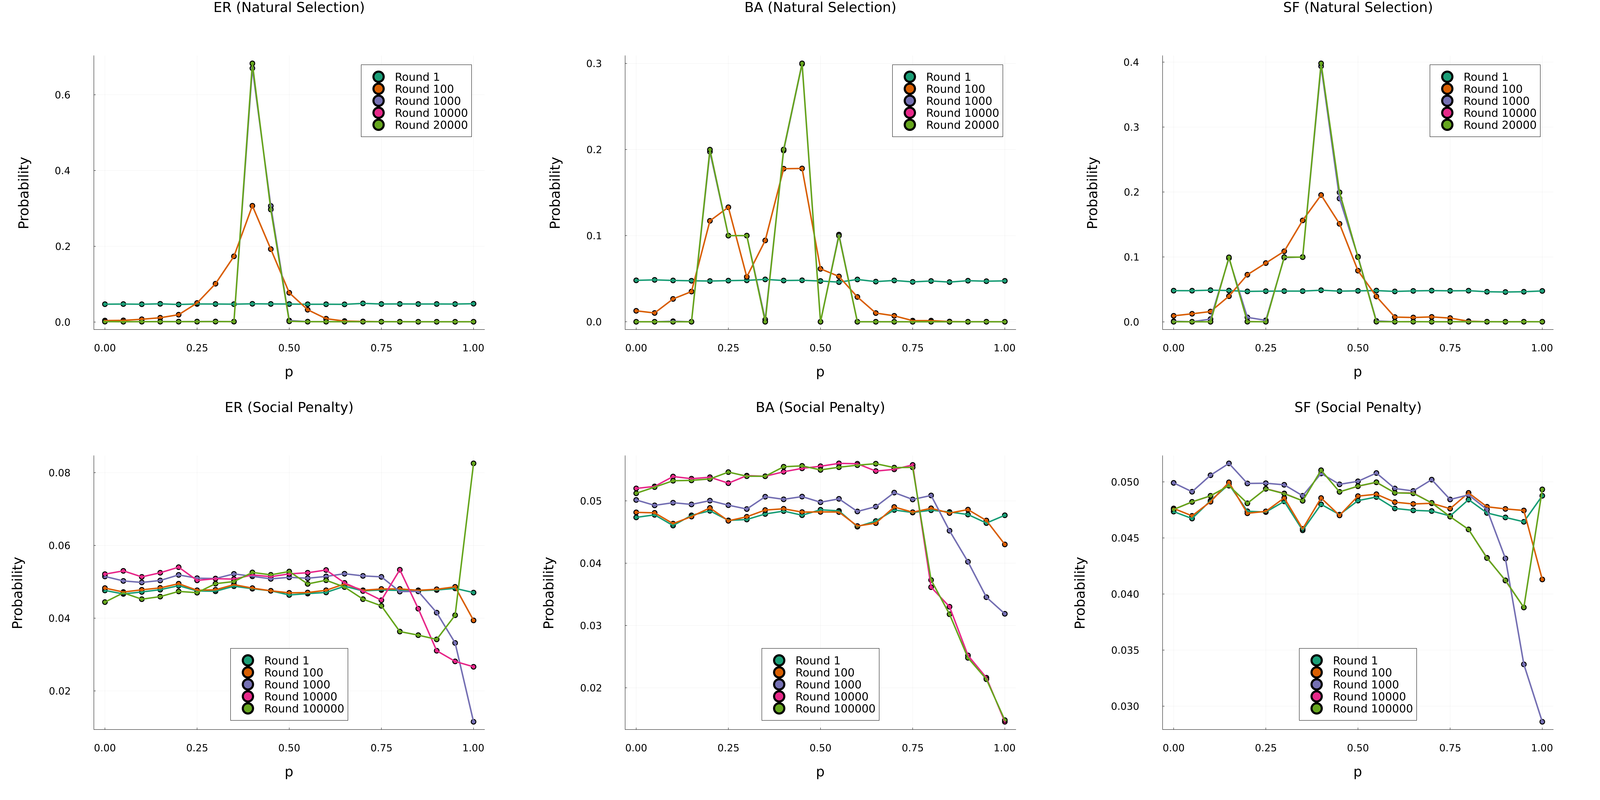
\includegraphics[width=1\textwidth]{images/Task34/TypeA_AllGraphs_AllRules.png}
    \caption{Networks with only type A players. The first row is with Natural Selection; the second row is with Social Penalty.}
\end{figure}

\begin{figure}[H]
    \centering
    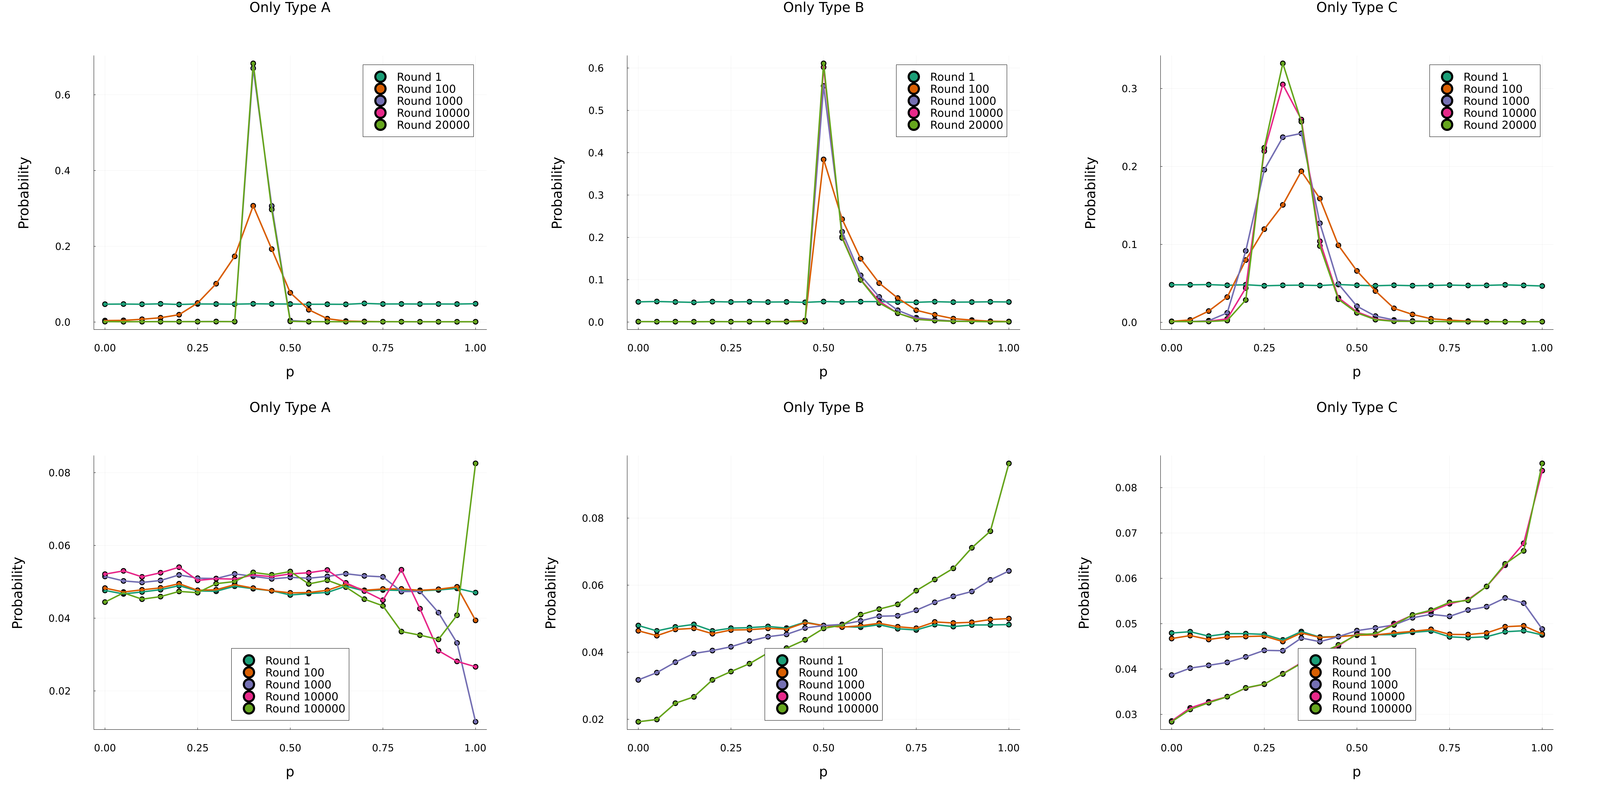
\includegraphics[width=1\textwidth]{images/Task34/AllTypes_Erdos_AllRules.png}
    \caption{Networks with all types of players on Erdos-Renyi networks. The first row is with Natural Selection; the second row is with Social Penalty.}
\end{figure}

As stated in \cite{UltimatumGame}, the change in topology does not massively change the distribution of strategies, but the updating rule does.
These results corroborate this conclusion. The individual distribution is different mainly because, in this task, a very low number of realizations was utilized.
\newpage